\chapter{RE-016 --- graphemeWidth Miscounts Emoji-Like Icon Characters}\label{record-402}

\noindent{\footnotesize\color{BookMuted}\path{docs/method/retro/RE_016-grapheme-width-miscounts-emoji-like-icons.md}\par}\smallskip

\begin{RecordMeta}
title: RE-016 — graphemeWidth Miscounts Emoji-Like Icon Characters
lane: retro
legend: RE

\end{RecordMeta}

\section{Disposition}\label{record-402-disposition}

Fixed on \texttt{r\allowbreak{}e\allowbreak{}l\allowbreak{}e\allowbreak{}a\allowbreak{}s\allowbreak{}e\allowbreak{}/\allowbreak{}v\allowbreak{}4\allowbreak{}.\allowbreak{}5\allowbreak{}.\allowbreak{}0} in commit \texttt{6\allowbreak{}9\allowbreak{}2\allowbreak{}9\allowbreak{}1\allowbreak{}f\allowbreak{}a}. First-party status icon paths now force text presentation with VS15 in core alerts, notes, overlay toasts, and notifications, and the grapheme regression coverage proves those symbols stay in the narrow text-width lane instead of drifting into emoji-width rendering.

\section{Original Proposal}\label{record-402-original-proposal}

\section{Summary}\label{record-402-summary}

\texttt{g\allowbreak{}r\allowbreak{}a\allowbreak{}p\allowbreak{}h\allowbreak{}e\allowbreak{}m\allowbreak{}e\allowbreak{}W\allowbreak{}i\allowbreak{}d\allowbreak{}t\allowbreak{}h\allowbreak{}(\allowbreak{})} in \texttt{p\allowbreak{}a\allowbreak{}c\allowbreak{}k\allowbreak{}a\allowbreak{}g\allowbreak{}e\allowbreak{}s\allowbreak{}/\allowbreak{}b\allowbreak{}i\allowbreak{}j\allowbreak{}o\allowbreak{}u\allowbreak{}/\allowbreak{}s\allowbreak{}r\allowbreak{}c\allowbreak{}/\allowbreak{}c\allowbreak{}o\allowbreak{}r\allowbreak{}e\allowbreak{}/\allowbreak{}t\allowbreak{}e\allowbreak{}x\allowbreak{}t\allowbreak{}/\allowbreak{}g\allowbreak{}r\allowbreak{}a\allowbreak{}p\allowbreak{}h\allowbreak{}e\allowbreak{}m\allowbreak{}e\allowbreak{}.\allowbreak{}t\allowbreak{}s} counts certain Unicode icon characters as 1 column wide, but many renderers (chat UIs, some terminal emulators, web-based terminals) display them as 2 columns wide. This causes box-drawing alignment to break when these characters appear inside bordered components.

\section{Affected Characters}\label{record-402-affected-characters}

\begin{center}
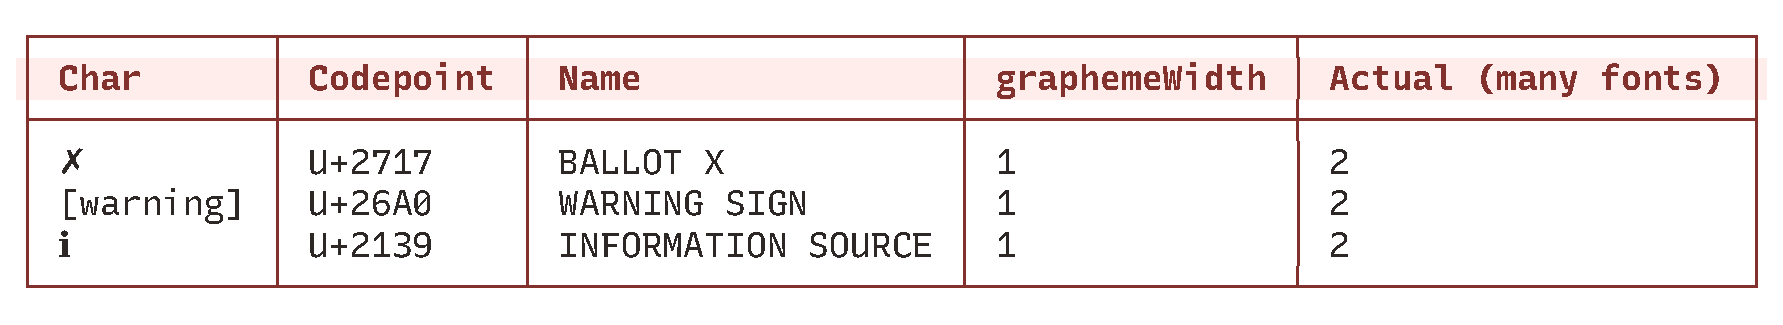
\includegraphics[width=\linewidth]{figures/tables/table-079-g1-1.pdf}
\par\smallskip{\scriptsize\color{BookMuted}Rows 1–3. Actual Bijou table component.}
\end{center}


\texttt{✓} (U+2713 CHECK MARK) renders as 1-wide in most contexts and is not affected.

\section{Symptom}\label{record-402-symptom}

The right border \texttt{│} of \texttt{a\allowbreak{}l\allowbreak{}e\allowbreak{}r\allowbreak{}t\allowbreak{}(\allowbreak{})} boxes is misaligned for \texttt{e\allowbreak{}r\allowbreak{}r\allowbreak{}o\allowbreak{}r}, \texttt{w\allowbreak{}a\allowbreak{}r\allowbreak{}n\allowbreak{}i\allowbreak{}n\allowbreak{}g}, and \texttt{i\allowbreak{}n\allowbreak{}f\allowbreak{}o} variants:

\begin{CodeBlock}
┌─────────────────────────────────────┐
│ ✗ Connection refused on port 5432. │   ← right │ doesn't reach ┐
└─────────────────────────────────────┘
\end{CodeBlock}

\section{Where It Matters}\label{record-402-where-it-matters}

\begin{itemize}
\tightlist
\item
  \texttt{a\allowbreak{}l\allowbreak{}e\allowbreak{}r\allowbreak{}t\allowbreak{}(\allowbreak{})} component --- uses \texttt{I\allowbreak{}C\allowbreak{}O\allowbreak{}N\allowbreak{}S} map with \texttt{✗}, \texttt{[\allowbreak{}w\allowbreak{}a\allowbreak{}r\allowbreak{}n\allowbreak{}i\allowbreak{}n\allowbreak{}g\allowbreak{}]}, \texttt{ℹ}
\item
  Any component that places these characters inside a \texttt{b\allowbreak{}o\allowbreak{}x\allowbreak{}(\allowbreak{})} or width-padded cell
\item
  Particularly visible in non-terminal monospace contexts (MCP chat output, web terminals, VS Code terminal)
\end{itemize}

\section{Files}\label{record-402-files}

\begin{itemize}
\tightlist
\item
  \texttt{p\allowbreak{}a\allowbreak{}c\allowbreak{}k\allowbreak{}a\allowbreak{}g\allowbreak{}e\allowbreak{}s\allowbreak{}/\allowbreak{}b\allowbreak{}i\allowbreak{}j\allowbreak{}o\allowbreak{}u\allowbreak{}/\allowbreak{}s\allowbreak{}r\allowbreak{}c\allowbreak{}/\allowbreak{}c\allowbreak{}o\allowbreak{}r\allowbreak{}e\allowbreak{}/\allowbreak{}t\allowbreak{}e\allowbreak{}x\allowbreak{}t\allowbreak{}/\allowbreak{}g\allowbreak{}r\allowbreak{}a\allowbreak{}p\allowbreak{}h\allowbreak{}e\allowbreak{}m\allowbreak{}e\allowbreak{}.\allowbreak{}t\allowbreak{}s} --- width calculation
\item
  \texttt{p\allowbreak{}a\allowbreak{}c\allowbreak{}k\allowbreak{}a\allowbreak{}g\allowbreak{}e\allowbreak{}s\allowbreak{}/\allowbreak{}b\allowbreak{}i\allowbreak{}j\allowbreak{}o\allowbreak{}u\allowbreak{}/\allowbreak{}s\allowbreak{}r\allowbreak{}c\allowbreak{}/\allowbreak{}c\allowbreak{}o\allowbreak{}r\allowbreak{}e\allowbreak{}/\allowbreak{}c\allowbreak{}o\allowbreak{}m\allowbreak{}p\allowbreak{}o\allowbreak{}n\allowbreak{}e\allowbreak{}n\allowbreak{}t\allowbreak{}s\allowbreak{}/\allowbreak{}a\allowbreak{}l\allowbreak{}e\allowbreak{}r\allowbreak{}t\allowbreak{}.\allowbreak{}t\allowbreak{}s} --- icon map (line 21-26)
\end{itemize}

\section{Options}\label{record-402-options}

\begin{enumerate}
\def\labelenumi{\arabic{enumi}.}
\tightlist
\item
  Fix \texttt{g\allowbreak{}r\allowbreak{}a\allowbreak{}p\allowbreak{}h\allowbreak{}e\allowbreak{}m\allowbreak{}e\allowbreak{}W\allowbreak{}i\allowbreak{}d\allowbreak{}t\allowbreak{}h\allowbreak{}(\allowbreak{})} to handle ambiguous-width characters correctly (hard --- width depends on the rendering context)
\item
  Replace the icons with ASCII-safe alternatives in a dedicated \texttt{p\allowbreak{}l\allowbreak{}a\allowbreak{}i\allowbreak{}n\allowbreak{}S\allowbreak{}t\allowbreak{}y\allowbreak{}l\allowbreak{}e} / MCP rendering path
\item
  Add a width-override mechanism so MCP context can declare these as 2-wide
\end{enumerate}

